%************VERSUCHSANORDNUNG*************
\section{Setup}
\label{sec:setup}
All experiments are set up on an optical table with a grid of positioning threads, using the designated mounts for the optical elements.
The grating spectrometer is connected to a PC, where its data is evaluated and plotted using APE Wavescan software. 
For optimal data collection, the laser beams orientation must be aligned using two points fixed in space.
These points are given by two optical apertures, localized in front of the mirror and at the entrance of the grating spectrometer, as seen in figure \ref{fig:execution:aperture}.

\subsection{Laser Source Characterization}
\noindent In figure \ref{fig:setup:power} the setup for measuring the average power of the laser is shown.
In figure \ref{fig:setup:basic} the central wavelength and the full width half maximum (FWHM) of the laser output is measured.
As the laser is expected to be in the infrared range, two BB1-E03 dielectric mirrors, which exceed 90\% reflectance in 750 - 1100 nm range, are chosen for wave guidance.


\begin{figure}[H]
    \centering
    \captionsetup{margin=3cm}
    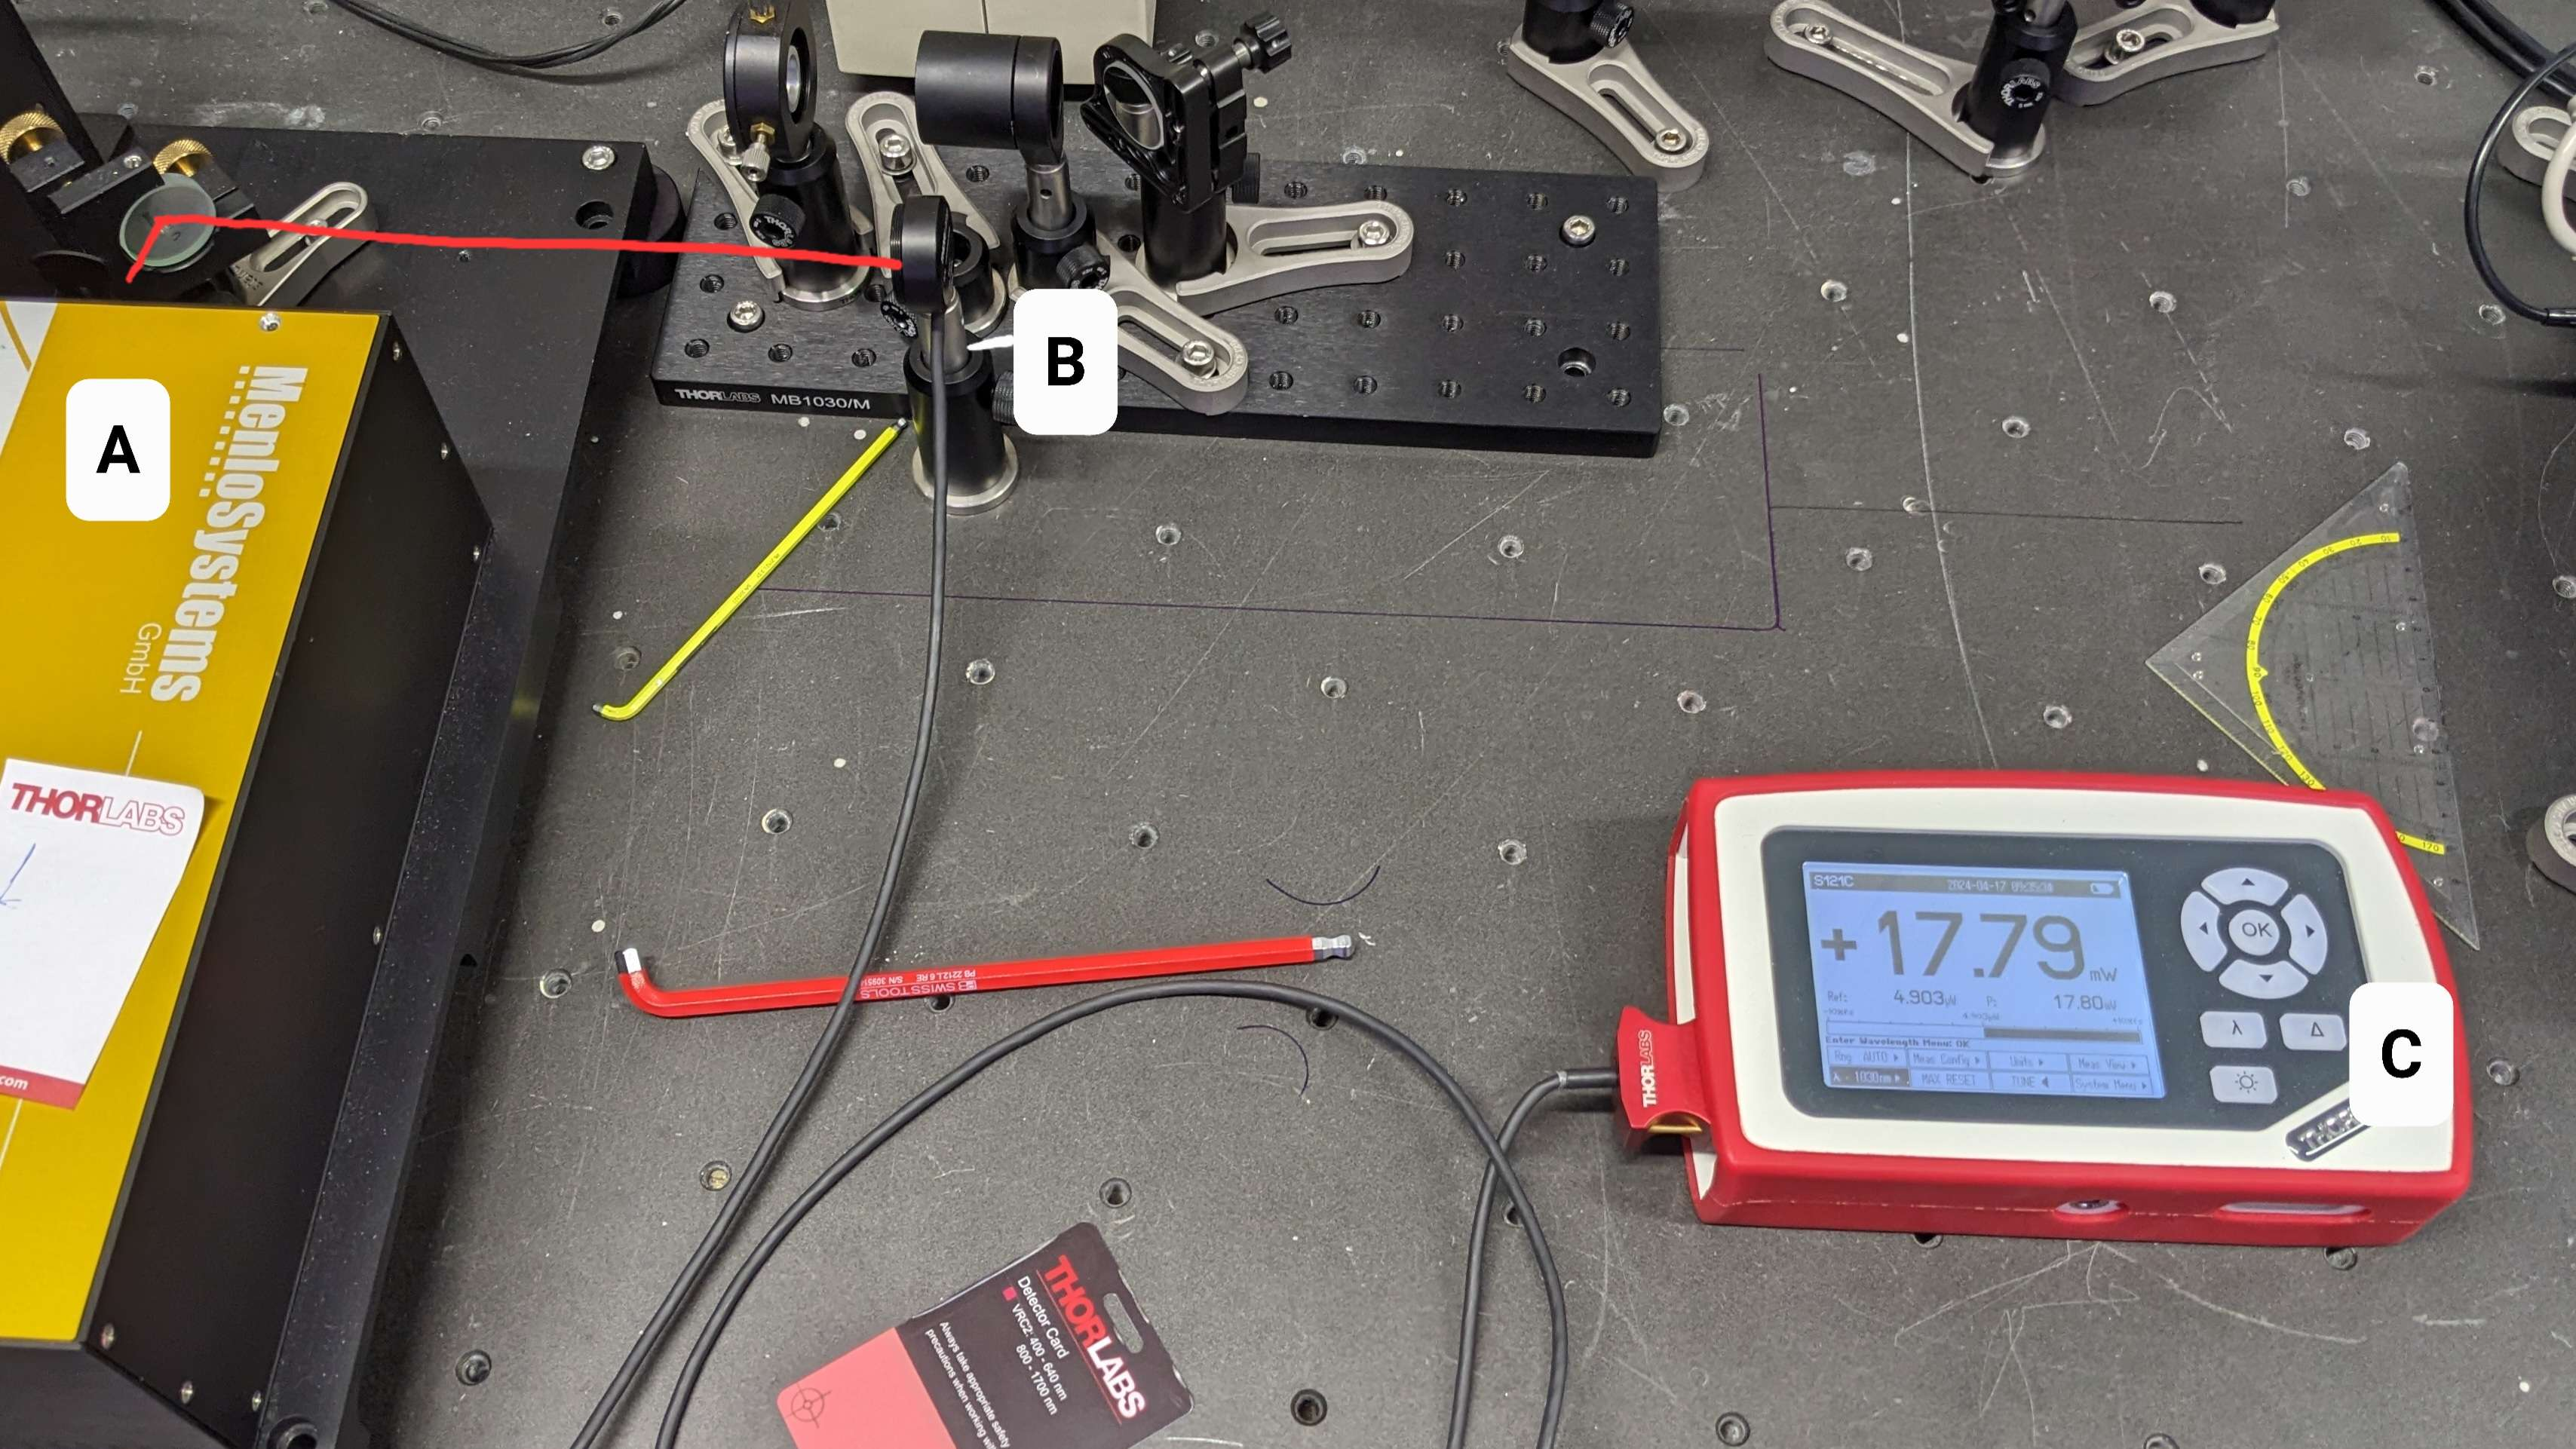
\includegraphics[width=0.7\textwidth]{laserpower.jpg}
    \caption{
        Characterization of a infrared laser via power meter: \\
        \textbf{A}: Femtosecond Ytterbium Laser, 
        \textbf{B}: Photodiode Sensor,
        \textbf{C}: Power Meter
    }
    \label{fig:setup:power}
\end{figure}
\begin{figure}[H]
    \centering
    \captionsetup{margin=3cm}
    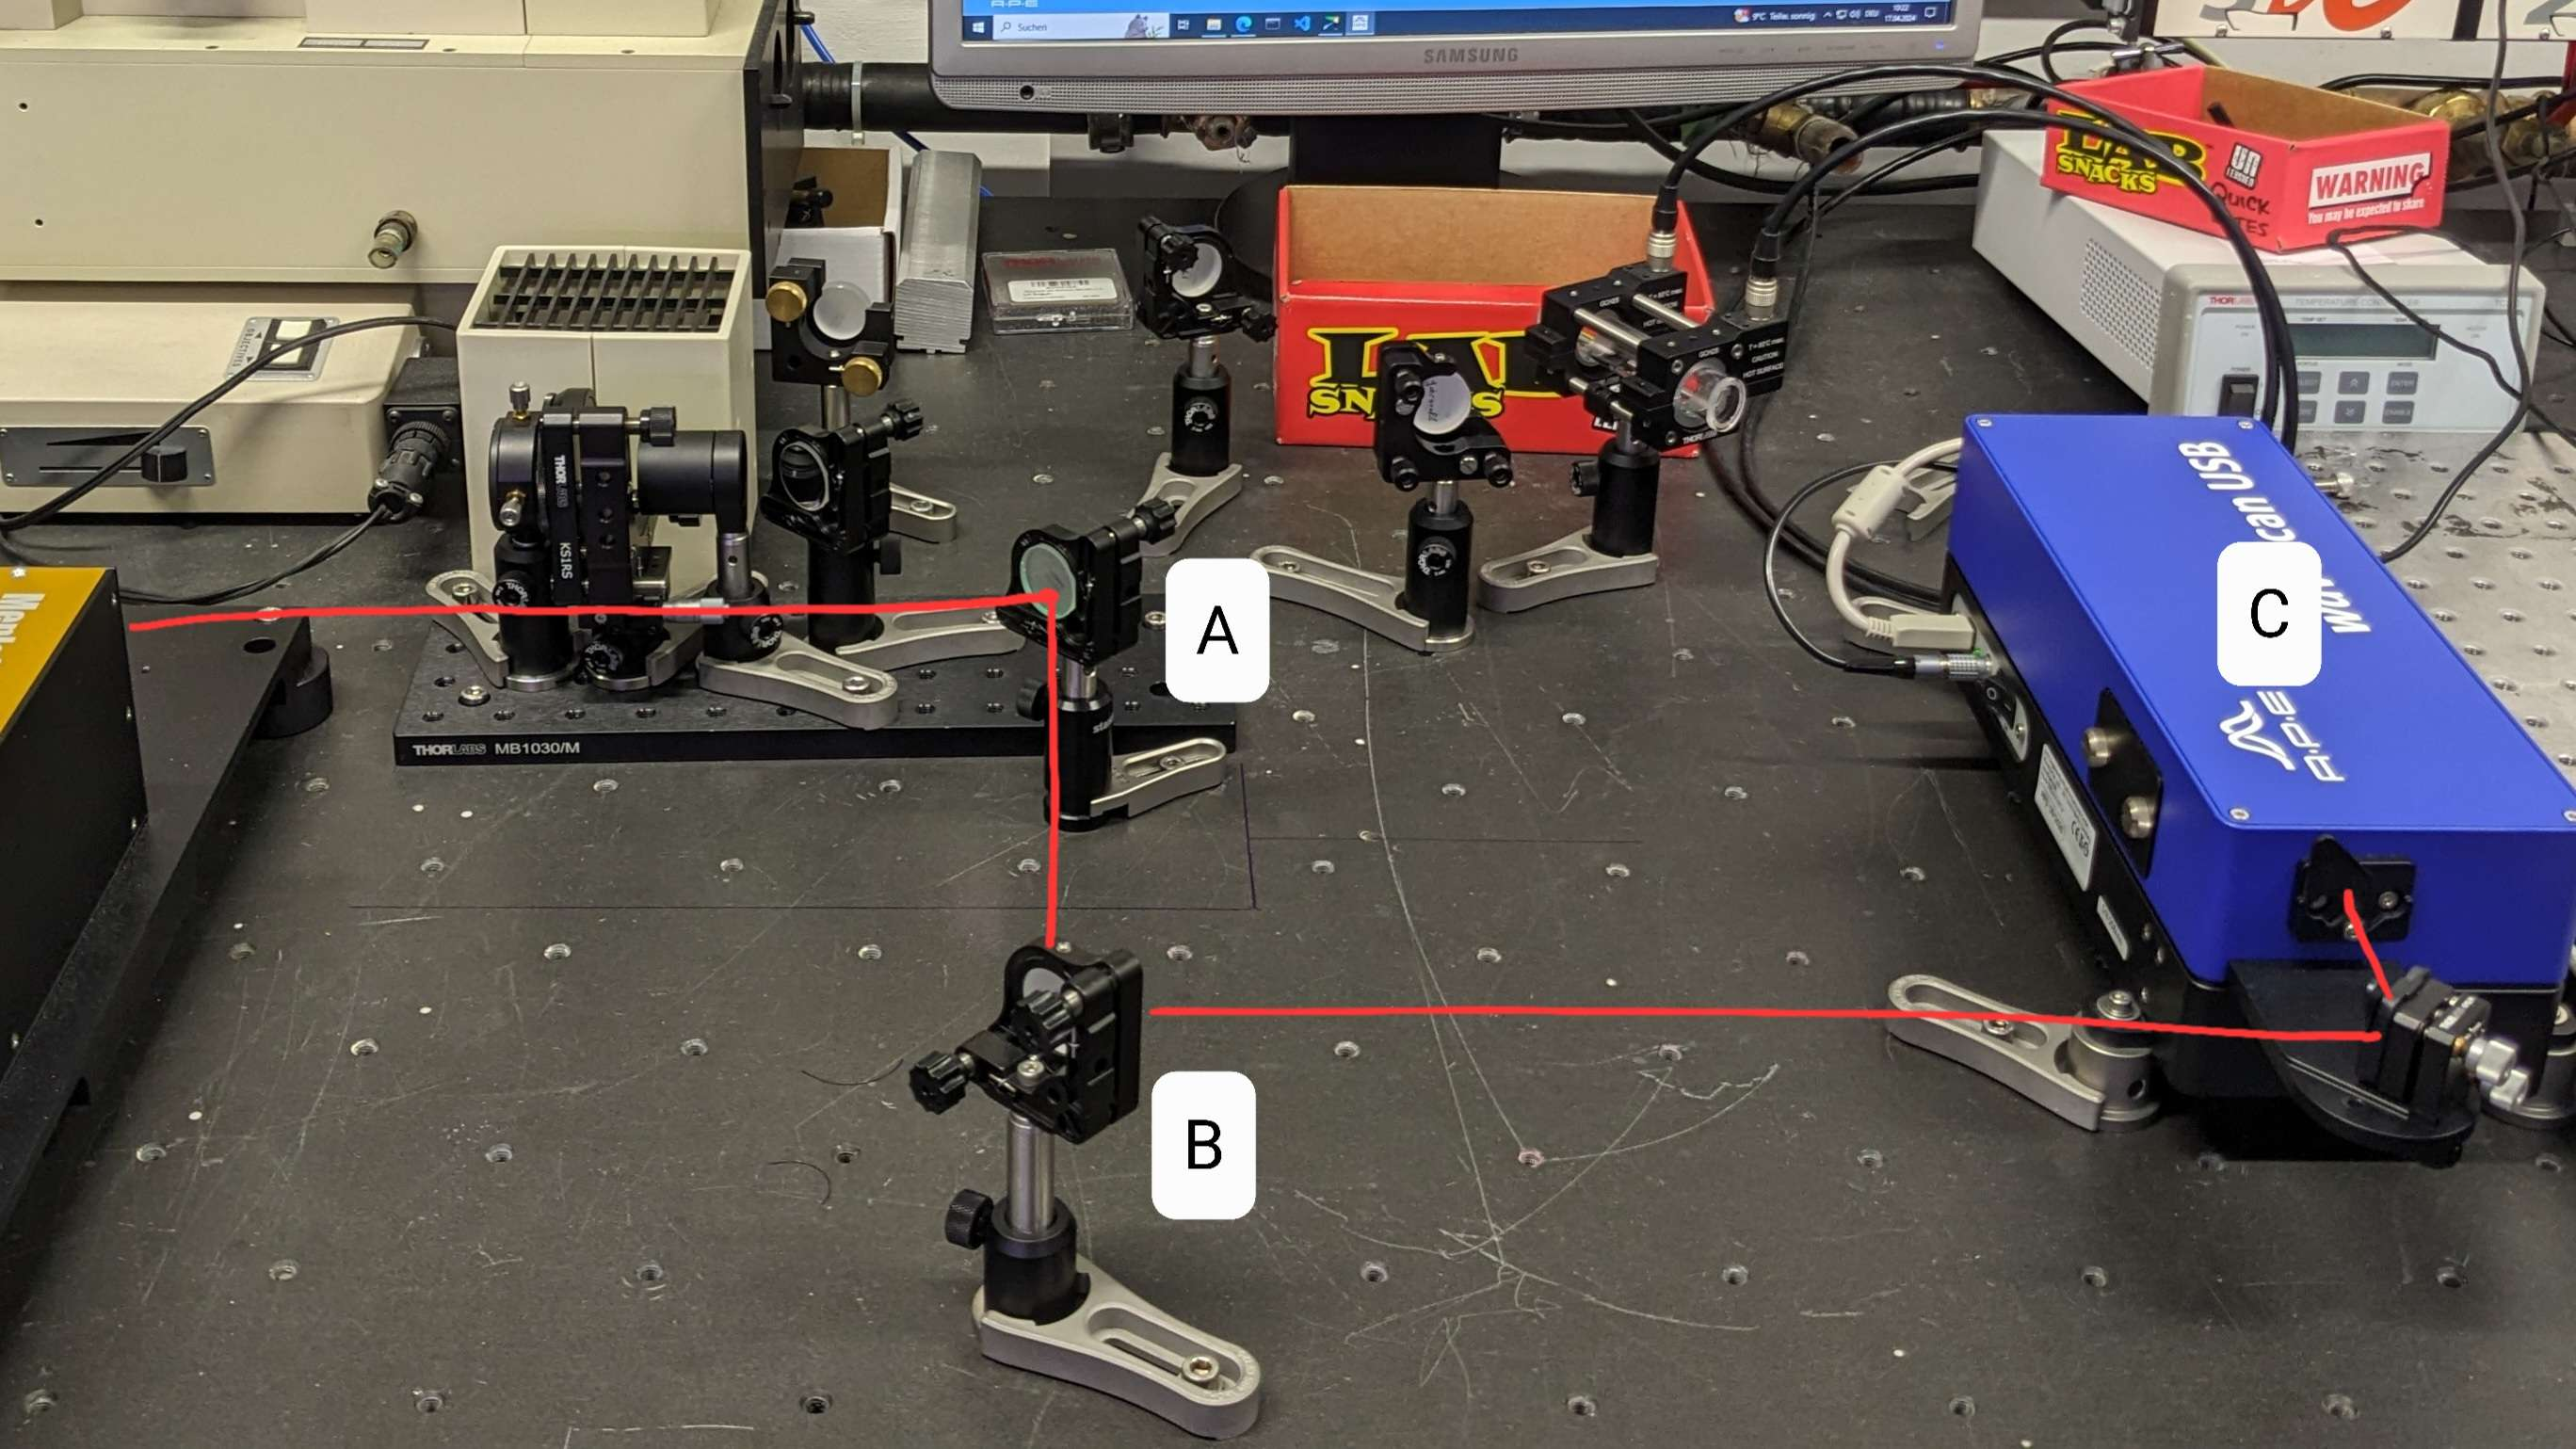
\includegraphics[width=0.7\textwidth]{graphics/basic-setup1.jpg}
    \caption{
        Characterization of a infrared laser via grating spectrometer: \\
        \textbf{A}: BB1-E03 Mirror,
        \textbf{B}: BB1-E03 Mirror,
        \textbf{C}: Grating Spectrometer
        }
        \label{fig:setup:basic}
    \end{figure}
    
\newpage
\subsection{SHG Characterization}
In this experiment a already ajusted second harmonic stage is introduced into the optical path. 
This stage consists of a collecting lens, a rotable Lithium Borate crystal and a collimator. 
The collecting lens focuses the laser on to the SHG-Crystal the and increases its power per area, which leads to more effiecient SH-generation.
By introducing a collimator after the SHG, one ensures maximal power at the grating spectrometer.
After the frequency doubling the laser is guided using BB1-E02 mirrors.
\begin{figure}[H]
    \centering
    \captionsetup{margin=3cm}
    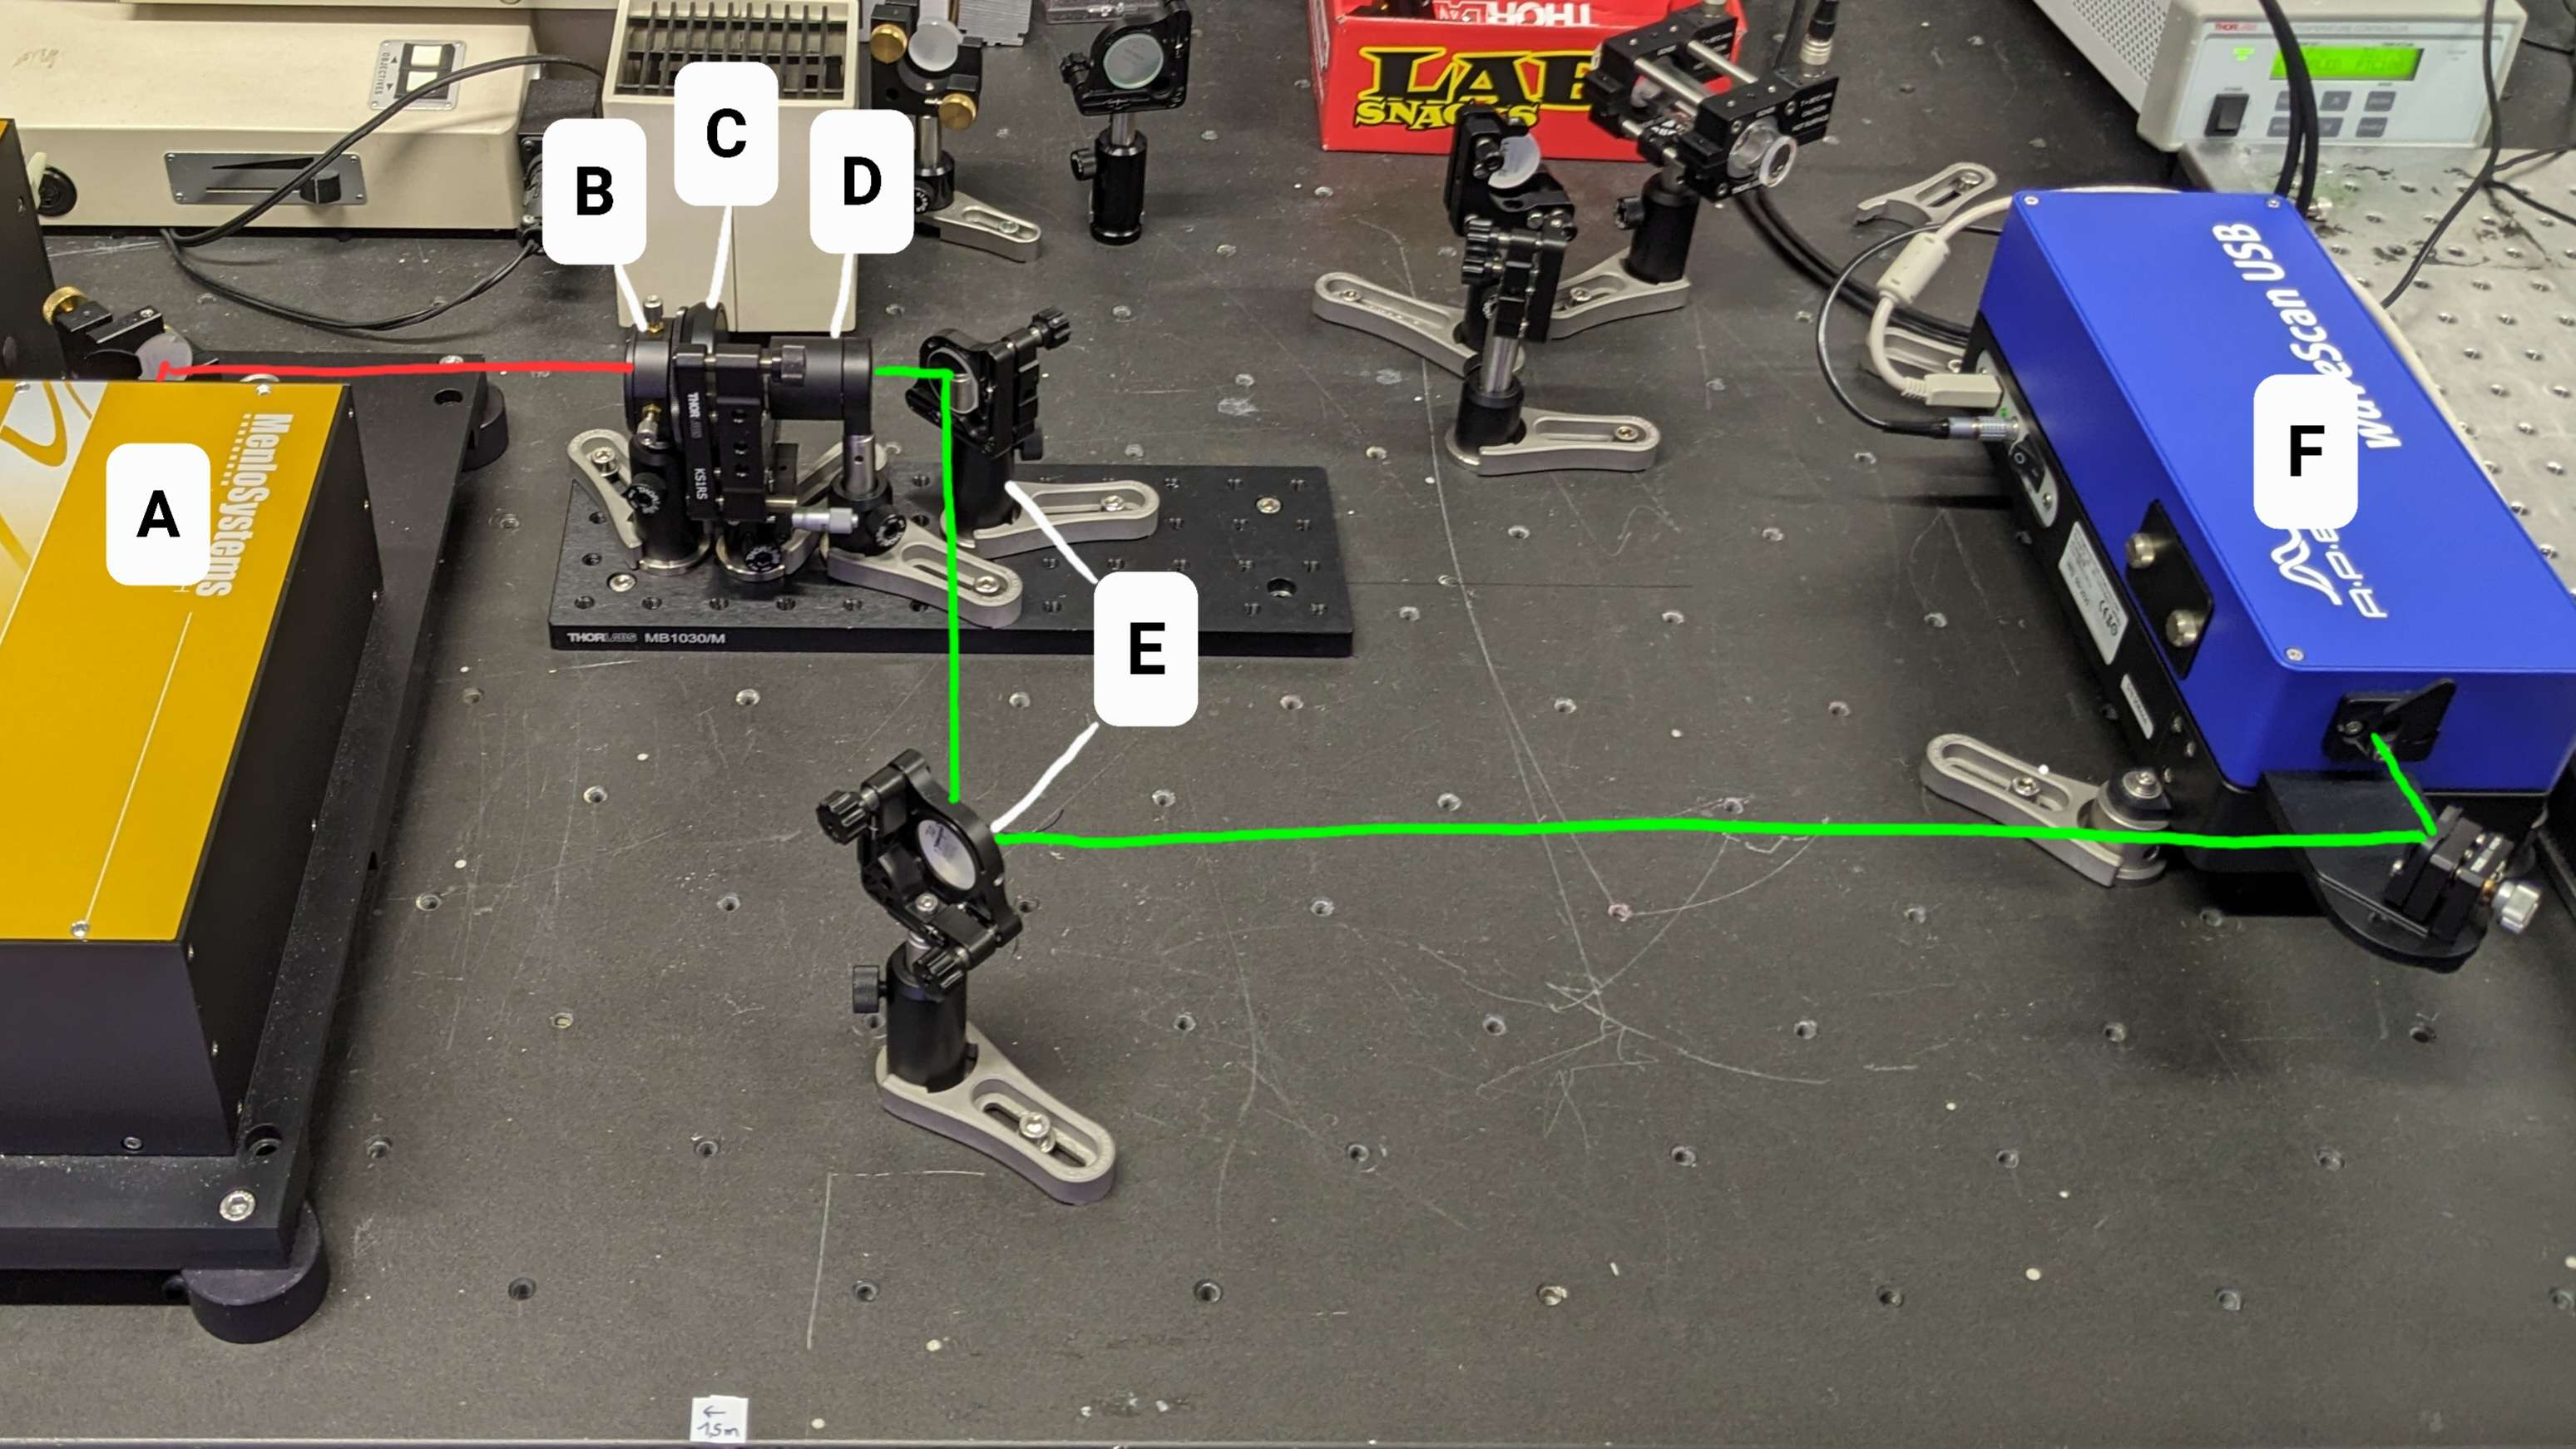
\includegraphics[width=0.7\textwidth]{graphics/shg-setup1.jpg}
    \caption{
        Setup of second harmonic generation (SHG) stage: \\
        \textbf{A}: Femtosecond Ytterbium Laser,
        \textbf{B}: Collecting Lens, 
        \textbf{C}: SHG - Crystal,
        \textbf{D}: Collimator Lens,
        \textbf{E}: BB1-E02 Mirrors,
        \textbf{F}: Grating Spectrometer
    }
    \label{fig:setup:shg}
\end{figure}
\subsection{Iodine Absorbance}
The SHG setup is expanded by introducing the iodine cell into the frequence doubled beam.
There are two variations of this experiment, which differ by the interaction lengths of the laser beam with the medium.
For a longer interaction length the laser is guided three times through the medium.
In the single pass setup the temperature is additionally varied.
The multiple pass setup is shown in figure \ref{fig:setup:iodine} ,the temperature controller is shown in figure \ref{fig:setup:temperature-controller}.
 
\begin{figure}[H]
    \centering
    \captionsetup{margin=3cm}
    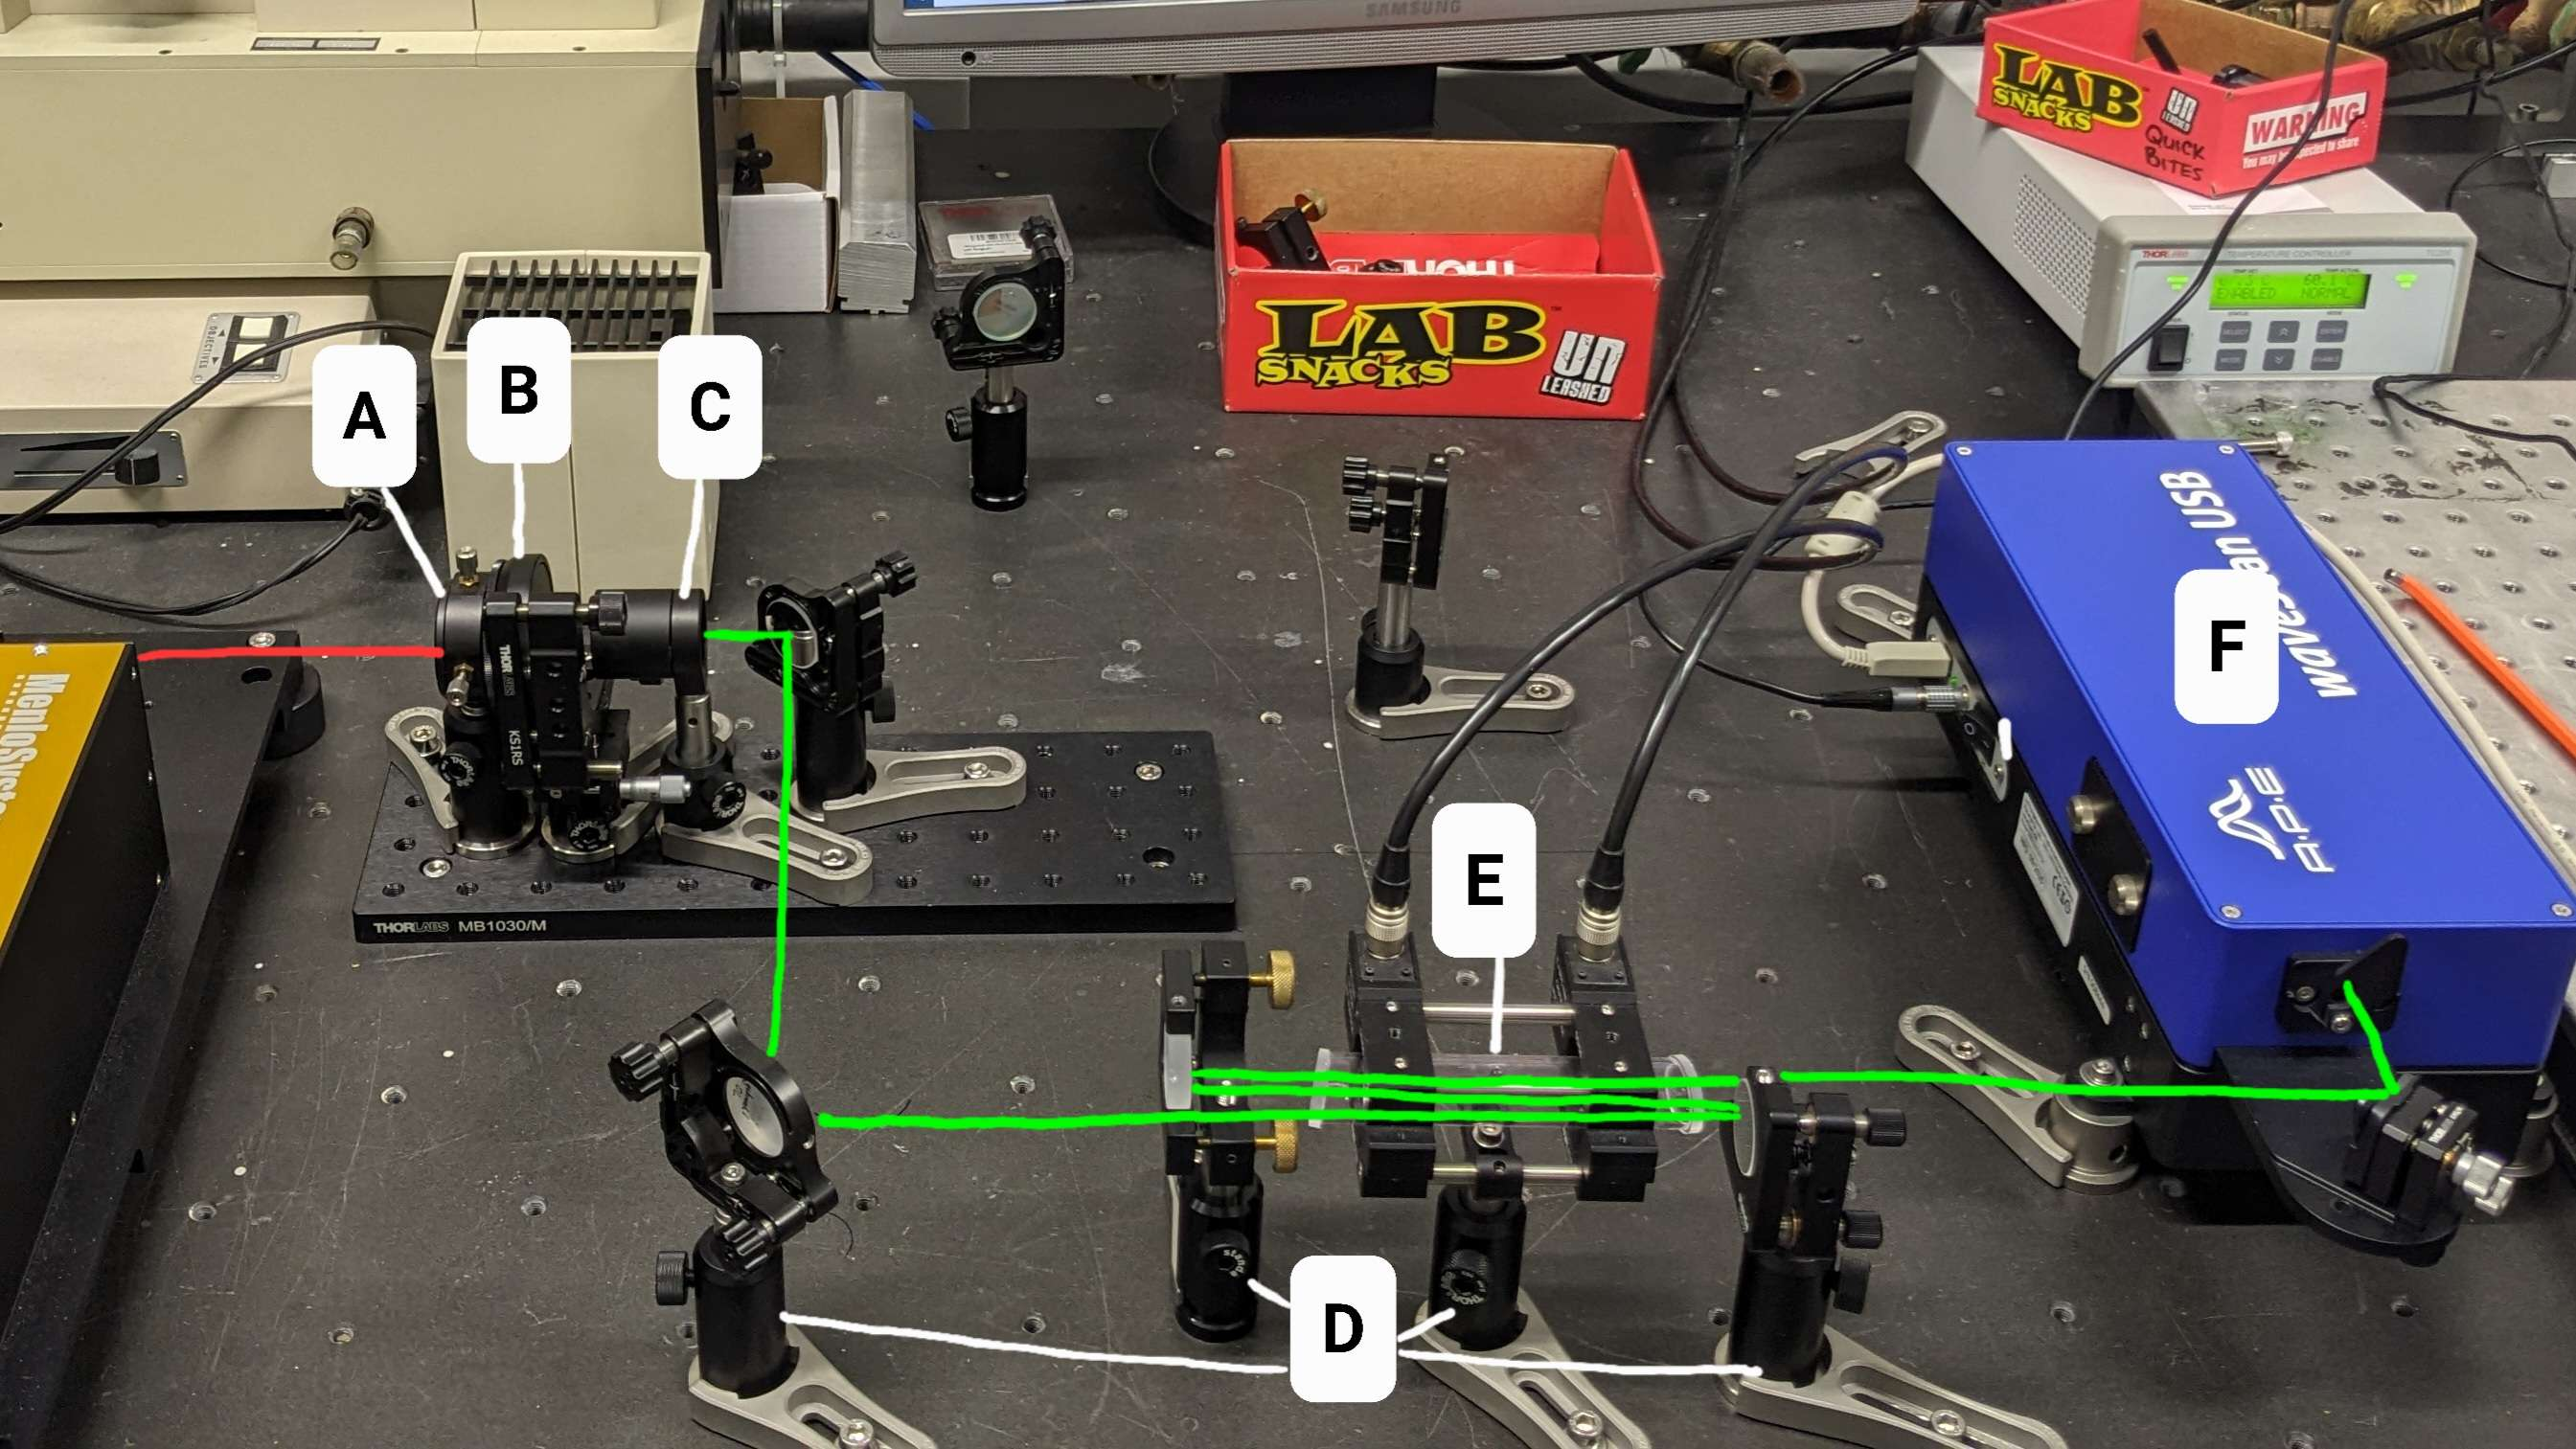
\includegraphics[width=0.7\textwidth]{graphics/iodine1.jpg}
    \caption{
        Setup for capturing the Absorbtion Spectrum of Iodine: \\
        \textbf{A}: Collecting Lens, 
        \textbf{B}: SHG - Crystal,
        \textbf{C}: Collimator Lens,
        \textbf{D}: BB1-E02 Mirrors,
        \textbf{E}: Iodine cell and heating element,
        \textbf{F}: Grating Spectrometer
    }
    \label{fig:setup:iodine}
\end{figure}

\begin{figure}[H]
    \centering
    \captionsetup{margin=3cm}
    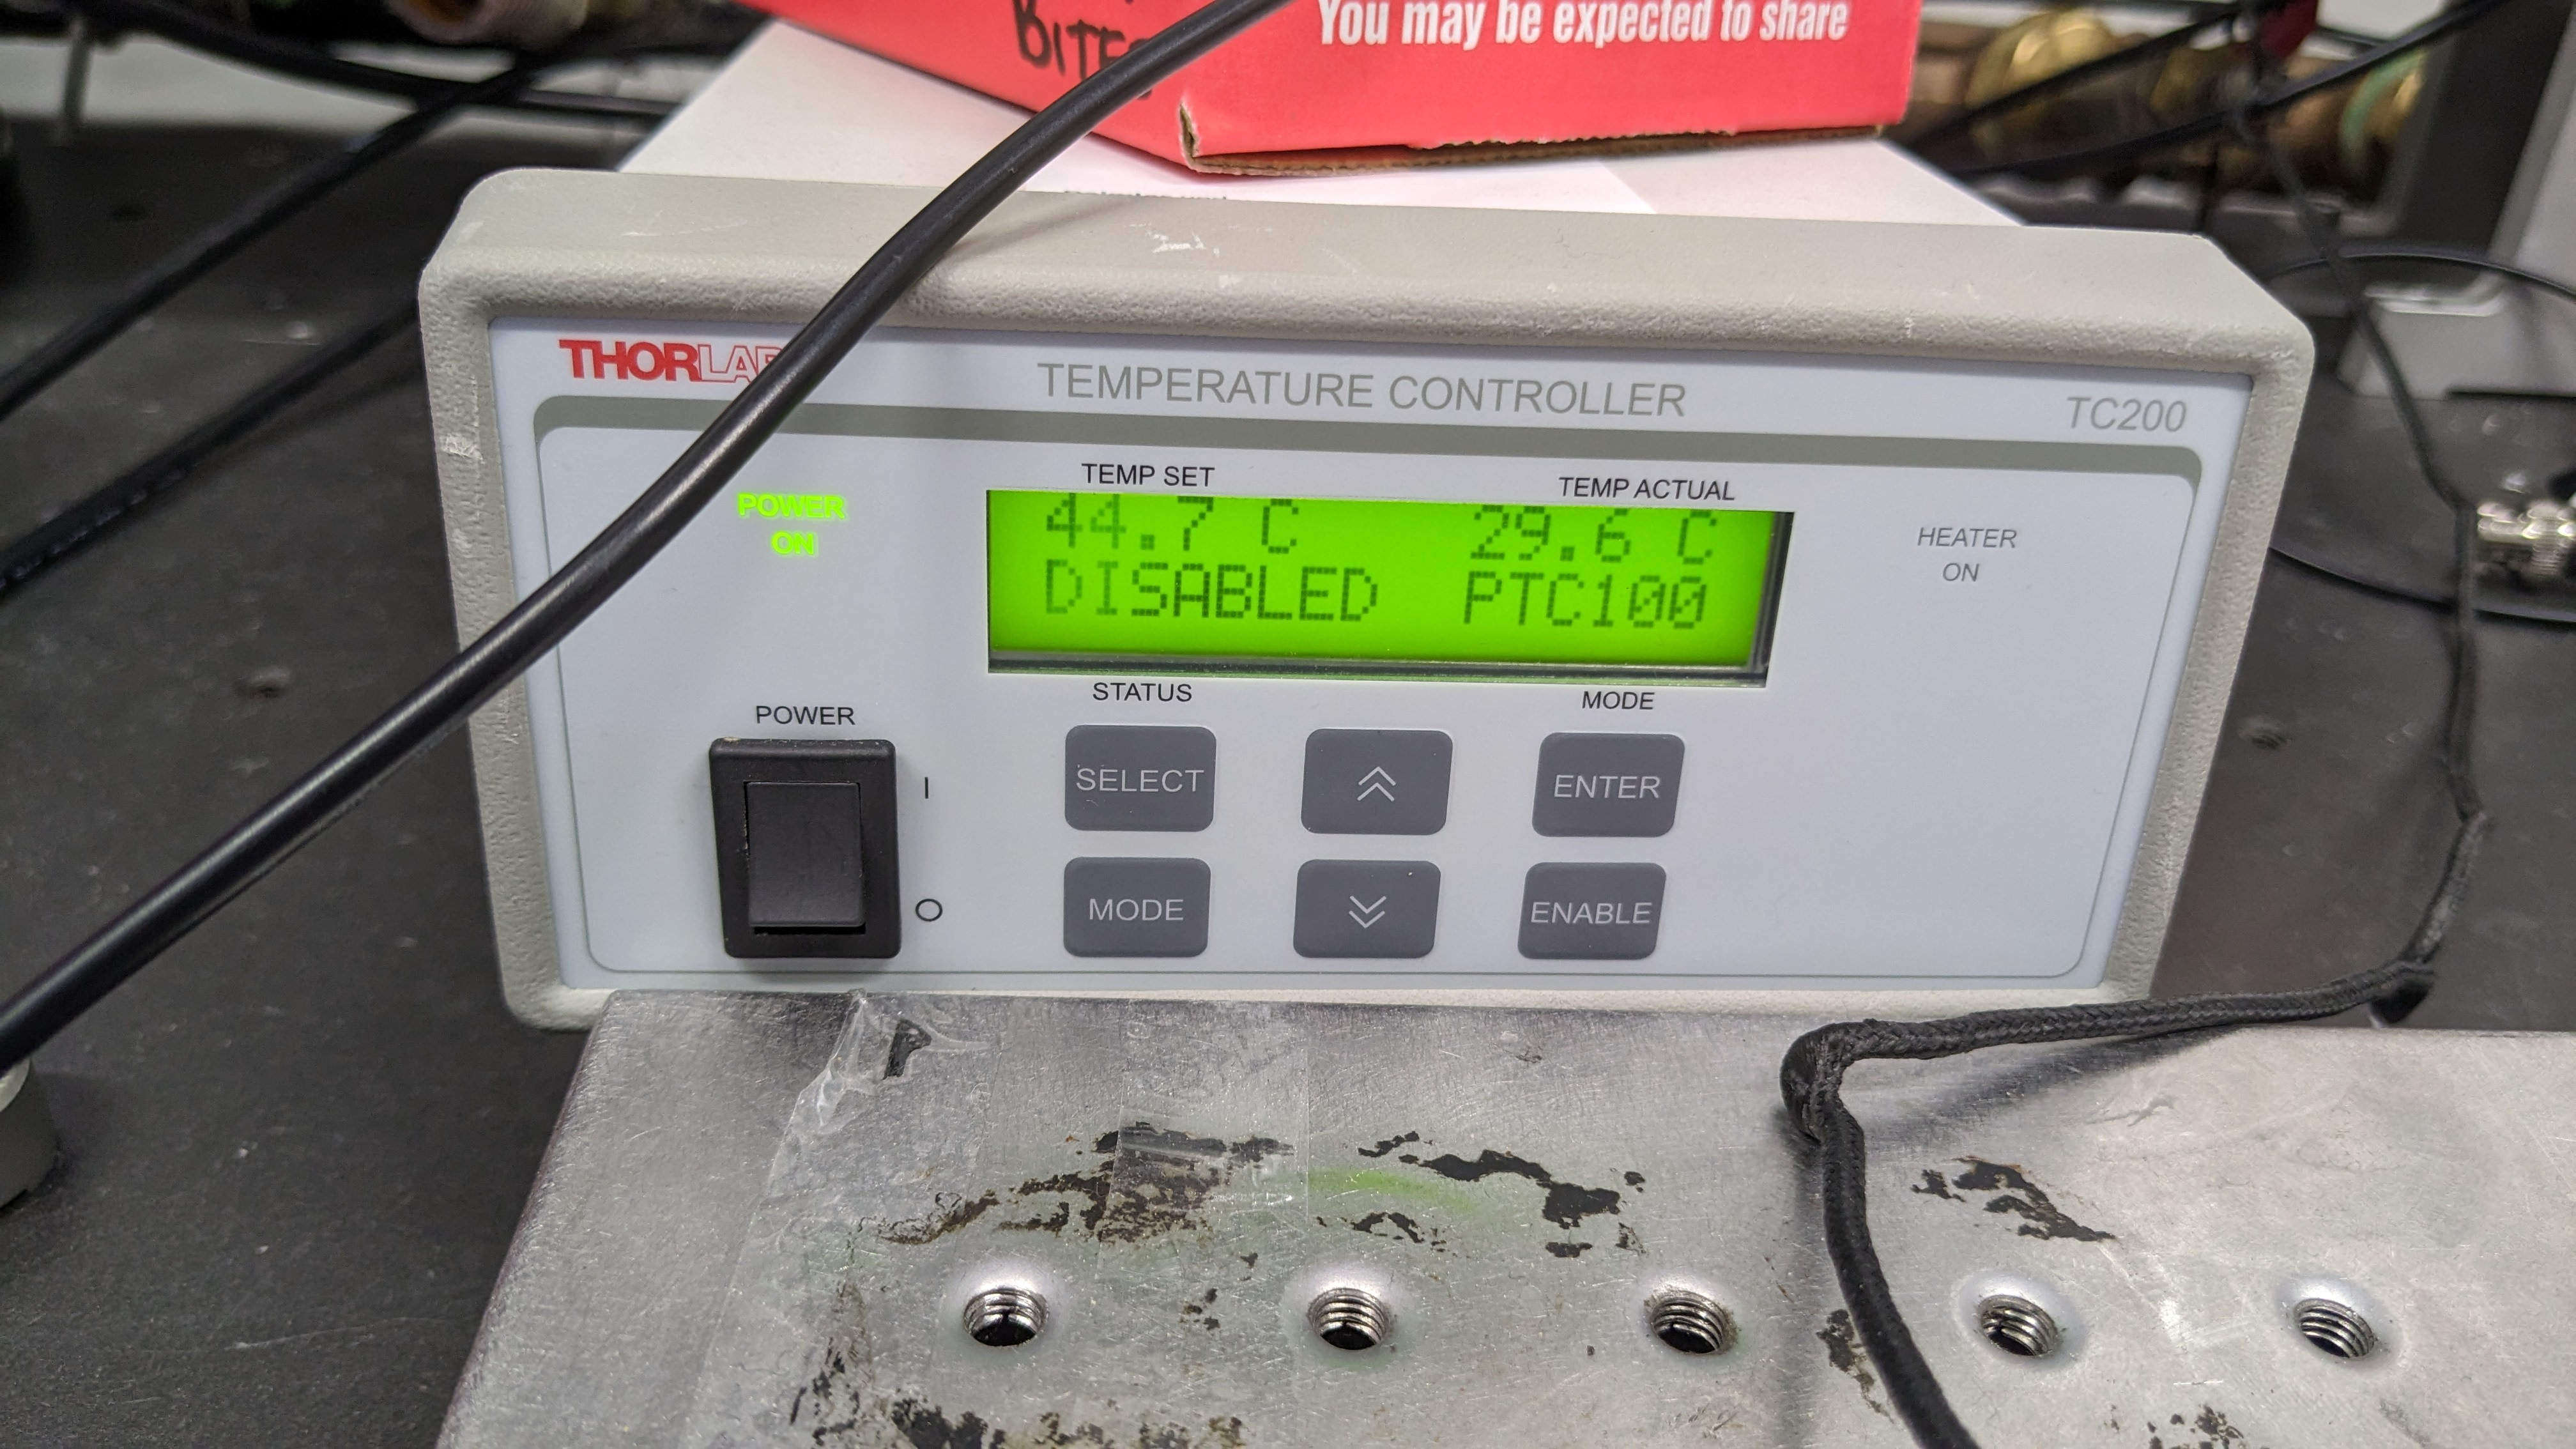
\includegraphics[width=0.7\textwidth]{graphics/temperature-controller.jpg}
    \caption{PID-Temperature Controller}
    \label{fig:setup:temperature-controller}
\end{figure}

\newpage